\documentclass{article}
%%%%%%% PACKAGES %%%%%%%%
\usepackage[utf8]{inputenc}
\usepackage[margin=3cm]{geometry}
\usepackage{graphicx}

\title{Software Engineering Project Architecture}
\author{Muhammad Azeem Haider $\mid$ Ali Asghar Yousuf \\
      Muhammad Shahid Mehmood $\mid$ Musab Sattar}
\date{\today}


\begin{document}

\maketitle

\section*{Introduction}

Thekedaar hatao is an application that aims to ease the process of building
your dream home. It provides the users with features that makes the building
process smoother and easier overall for the user of the application. The
calculator on the application, will provide you with an estimated amount of
cement, cinder blocks, sand, and other such raw materials that are essential
while building your house. In addition, the application will help cater the
dreamers by having a forum where people can communicate about the problems that
have arisen and how they tackled them. Advice threads and asking for help will
be carried out on the forum. Since you can never be sure of how much material
you exactly need, there is always a (+ or -)5\% chance of having extra
material, you can also sell this to other users on the app through a buy and
sell section. For individuals wanting to have a communication privately, the
application will also provide an opportunity to privately chat with someone
registered on the application.

\section*{Requirements}

\subsubsection*{Functional}

\begin{enumerate}
      \item \textbf{Login}

            Our App will let users login with their email as well as with google.

      \item \textbf{Raw Material Calculator}
      
            In the app, users can calculate the amount of raw material required for building based on their square footage.

      \item \textbf{Forum}
      
            Users can interact with other consumers and discuss their problems on a moderated forum, which could also be referred by users having similar queries/problems.

      \item \textbf{Market Place}
      
            A place where users can connect with reputable vendors.

      \item \textbf{Chat}
      
            A personal chat with other users/vendors so they can talk and make deals privately.
\end{enumerate}

\subsubsection*{Non-Functional}

\begin{enumerate}

      \item \textbf{Performance}

            The application will run smoothly on all devices supporting IOS 15 (and above)
            or Android 10 (and above). The application would not be resource intensive thus
            the performance would be enhanced.

      \item \textbf{Aesthetic}

            The aesthetic of the application will be developed in a way where it will make
            it easy for the users of the application to use it efficiently. The different
            features of the application will be inter-connected in a manner that will make
            the application a useful addition.

      \item \textbf{Usability}

            The mobile application will be usable in the sense that it will be easy for
            people of all ages to use the application for their benefit. The calculator,
            forum, marketplace, and chat messaging will all be easy to use.

      \item \textbf{Compatability}

            The application will be compatible with all mobile phones supporting the
            recommended operating system.

      \item \textbf{Reliability}

            The application will be reliable in the sense that it will not crash for users
            when they are using it. The application will also be reliable as it will always
            provide the perfect solution to the best of the applications knowledge.

      \item \textbf{Security}

            The user details submitted at the time of sign up to the application will be
            secure and will not be released to the public at any time.

\end{enumerate}

\section*{Use Cases}

\subsubsection*{Explanation}

There are two actors in our class diagram. Our primary actor in the class
diagram is the user of the application. The admins of the application that will
manage the application will be the secondary actors of the application. The
users will be concerned with the five features of the application that are;

\begin{itemize}
      \item Login and/or Signup
      \item Raw Material Calculator
      \item Forum
      \item Private chat
      \item Marketplace
\end{itemize}

The user will first sign up to the application, if the user is already
registered to the application, he/she will login to the application. The user
will also use raw material calculator in which one can input the amount of land
in sq/ft and get an estimation on how much raw material might be needed. In
addition, they will also be concerned with the marketplace. The users will be
divided into two types in the marketplace. The vendors that will sell the raw
material, and the consumers that will buy the raw material. The forum and the
chat will be administered by the admins as to stop anyone from misbehaving on
the public forums. The user will also have to set their profile and will have
to verify.

\newpage

\subsubsection*{UML Diagram}

\begin{figure}[!h]
      \begin{center}
            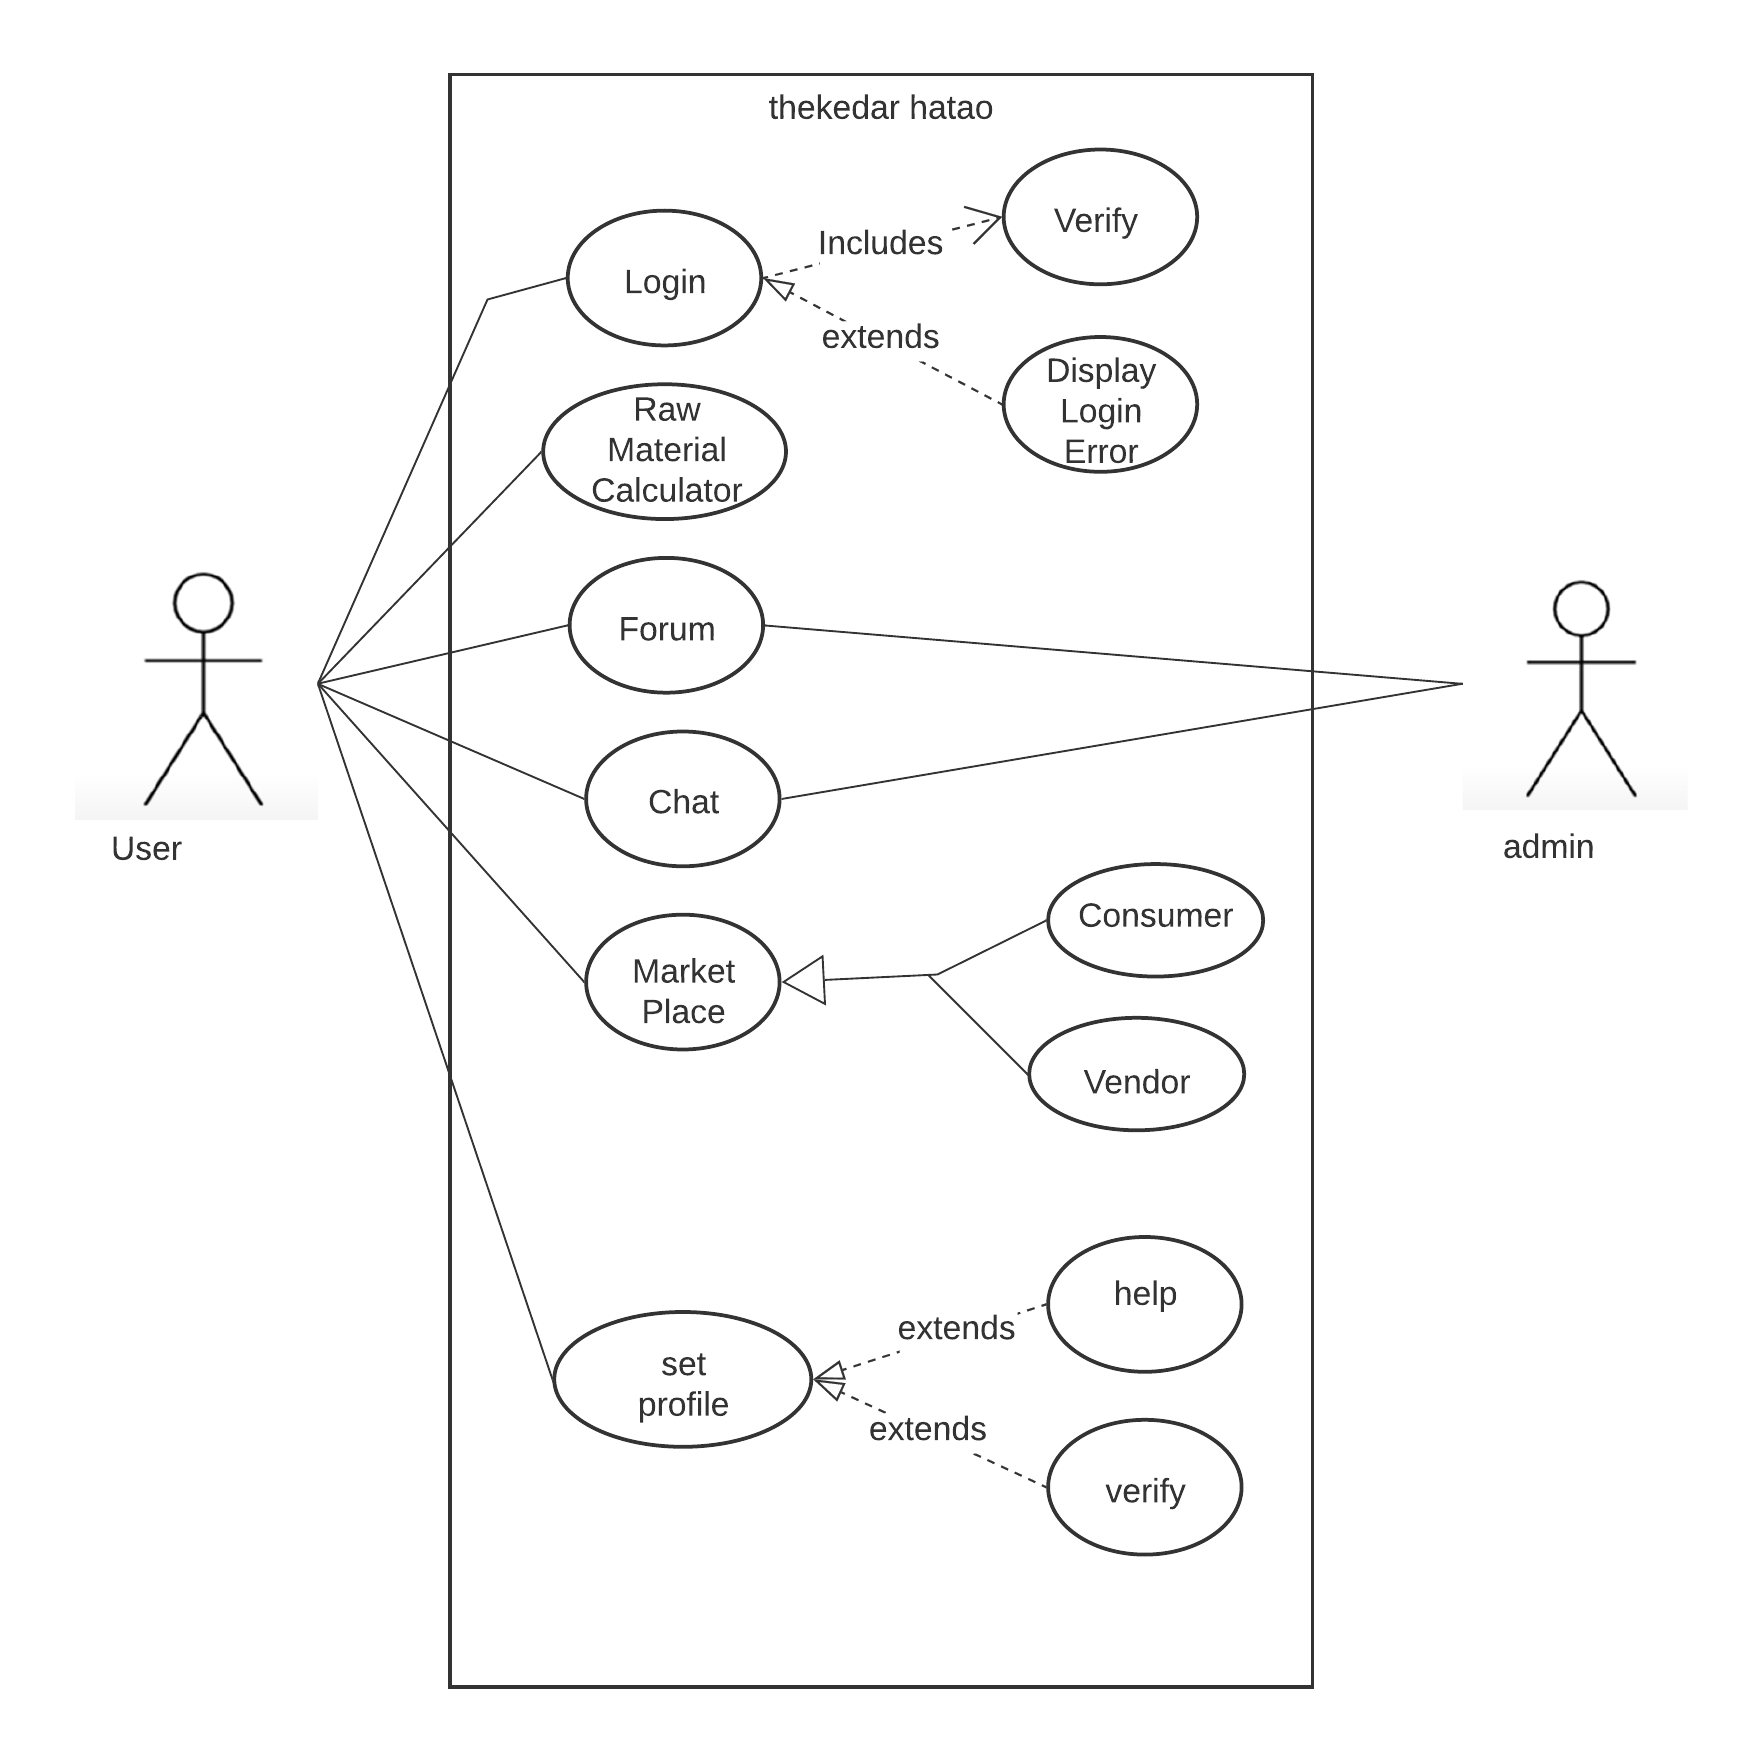
\includegraphics[width=1\linewidth]{usecase.png}
            \caption{usecase}
            \label{fig:UML}
      \end{center}
\end{figure}

\newpage

\section*{Sequence Diagrams}
\centering
\begin{figure}[!h]
      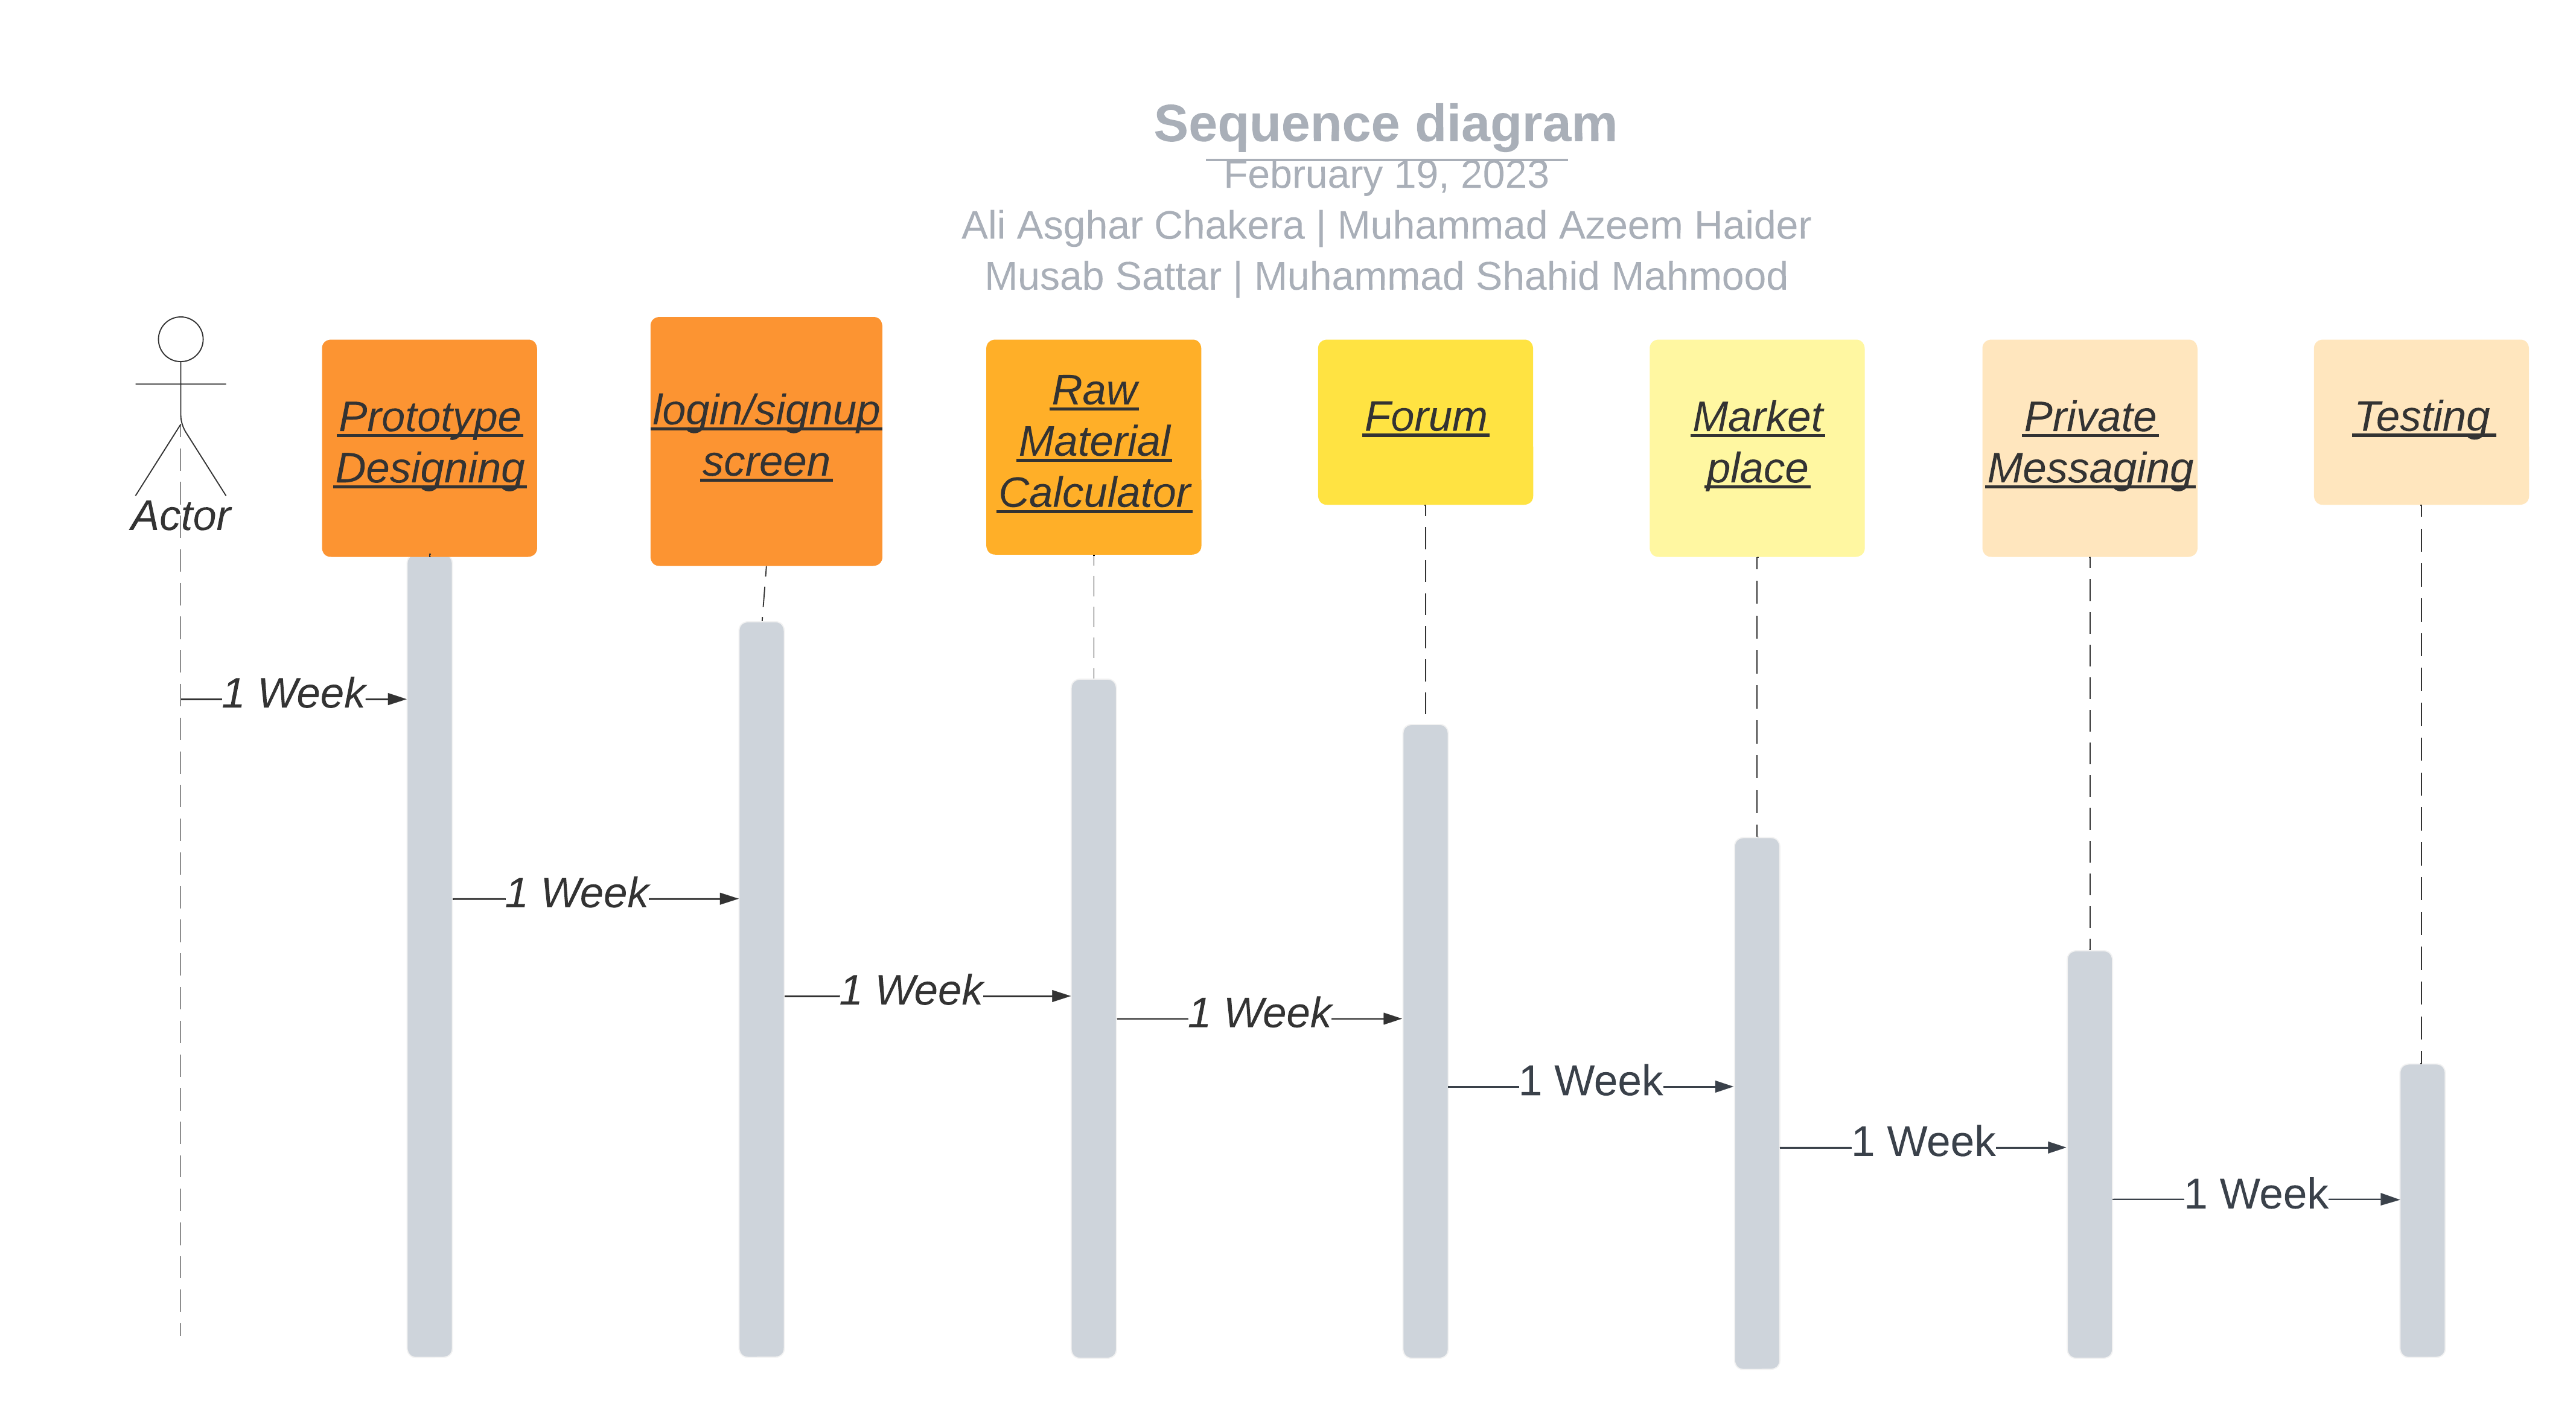
\includegraphics[width=1\linewidth]{Sequence diagram.png}
      \caption{Sequence Diagram}
      \label{fig:seq}
\end{figure}

\end{document}